\subsection{Annexes}
Lien GitHub pour télécharger les sources LaTeX : 
\url{https://github.com/blackjack-nix/stage_E1.git}
\subsubsection{Organigramme de l'IFSEM}
\centerline{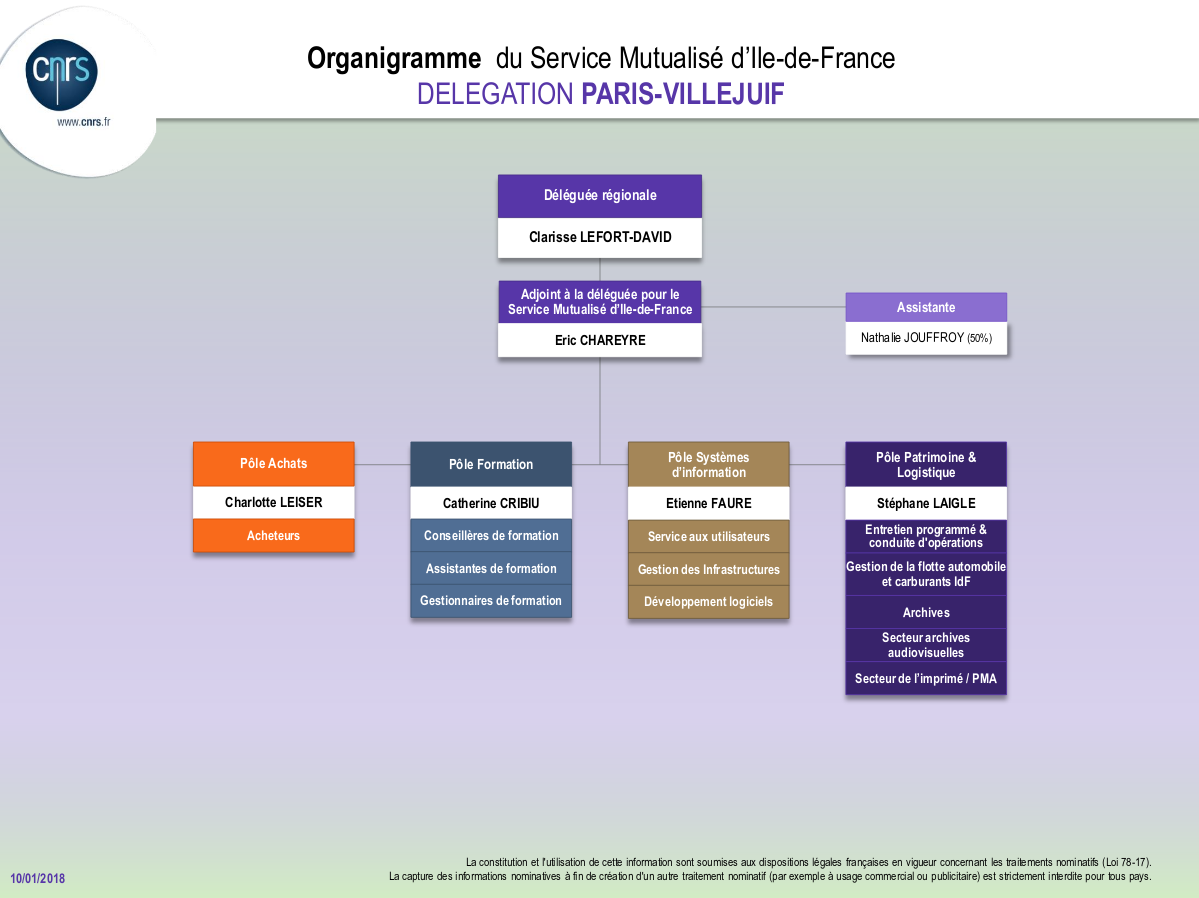
\includegraphics[width=15cm]{./images/ifsemorga.png}}

\subsection{Sources}
\begin{itemize}
    \item \url{http://www.cnrs.fr/}
    \item \url{https://www.dr1.cnrs.fr/spip.php?rubrique59}
    \item \url{https://fr.wikipedia.org/wiki/Centre_national_de_la_recherche_scientifique}
    \item \url{https://otrs.com/product-otrs/}
    \item \url{https://www.dr1.cnrs.fr/spip.php?article180}
    \item \url{https://blog.misterbean.fr/machine-cafe-entreprise}
    \item \url{https://www.quest.com/fr-fr/products/kace-systems-management-appliance/}
\end{itemize}
\newpage
\subsection{Attestation de fin de stage}
\newpage
\subsection{Ordre de mission}
Comme expliqué en partie 3.1.2, j'ai dû me déplacer sur le campus de Meudon. J'ai donc demandé un d'ordre de mission que voici :
\\
\\
\textit{
Bonjour,\\
Je soussigné Etienne FAURE, responsable du pôle SI de l’IFSeM, atteste que Théo \\PERESSE-GOURBIL actuellement stagiaire de 1ere année de l’ESIEE Paris effectuera un déplacement professionnel à la délégation Régionale du CNRS à Meudon (92) le jeudi 18 juillet 2019 pour la journée.
\medbreak
Pour faire valoir ce que de droit.
\smallbreak
Etienne FAURE}
\subsection{Remerciements}
A l'issue de ce stage, je tiens à remercier Mr Éric WIRTH et tous les professeurs de l'unité P\up{5} pour m'avoir permis de rédiger CVs et lettres de motivations ainsi que dans la recherche ce stage. 
\smallbreak
Je voudrais sincèrement remercier Mr Etienne FAURE, responsable du pôle SI de l'IFSeM qui fut aussi mon tuteur de stage pour avoir accepté de m'accueillir dans cette entreprise et de réaliser ce stage qui fut très formateur.
\smallbreak
Je souhaiterais aussi remercier tout l'IFSeM pour m'avoir rapidement intégré au sein du groupe, en particulier Baptiste BARAKOWSKY, Louis HERMEL et Vincent ROBERT qui m'ont accueilli dans leur bureau et avec qui j'ai passé ce mois. Ils ont su rendre ce stage intéressant et enrichissant d'un point de vu personnel et professionnel.